%%Relayattack part in the article on PKE

\subsection{Relayattacks}
\label{sec:relayAttacks}
\subsubsection*{Idea}
%Describe attack idea
	As described before relay attacks base on the problem of localization in
	wireless networks.
	Attacking a passive Key-less entry system,
	the attacker relays the probing signal emitted from the car to the victims
	customer identification device (CID).
	The CID the emits a signal that opens the doors of the vehicle.
	Now the attacker can enter the car and again relay the signals emitted by the
	car so that he can ignite the engine.
	
	This method has been practically tested on different PKE systems by \cite{relayAttacksFranc}. %TODO \citea{} %DER Artikel
	The authors show that it is an easy and feasible attack.
	It also does not require very specialized hard- or software and
	the required components can be easily aquired with a relatively small budget.
	The relay attack is transarparent to any higher layer cryptography,	%transport layer?
	and so it can easily circumvent the security systems of most PKE systems.

\subsubsection*{Variants}
	There are some variants in attacking PKE systems.
	Altough the attack could be in principle be carried out by one attacker alone,
	the literature usually asumes at least two attackers.

%two thieves
	\label{par:twoThieves}
	Having \textsl{two thieves} performing a relay attack,
	the roles are split.
	The first thieves will try to get close to the victim and place
	the sending device close to the victims CID.
	This could take place in a store,
	where it doesnt raise attention to the victim if the attacker
	is in range of the CID.
	The second thief will be near the car,
	probably parked on the stores own carlot,
	to capture its probing signals.

	Now the signals are relayed between the CID and thse car,
	and the car might open and start,
	allowing the second thiee to drive away.
	
%three thieves	
	\label{par:threeThieves}
	\citeauthor{someAttacksPKES} also describe an attack carried out by three thieves.
	This more complicate attack involves using seperate frequencies to transmit the signals
	from the vehicle to the CID and vice versa.
	The attack is not vulnerable to the introduction of a feedback loop,
	because thief 1 and thief 3 approach the vehicle from opposite directions,
	so that they do not pick up the signals emitted from their relaying antennas.
	Thief 2 is near the CID to pick up and relay the signals to theif 1 and 3.

\subsubsection*{Material \& Methods}
	\label{sec:matmet}
	This Section refers to the publication of \citeauthor{relayAttacksFranc} from \citeyear{relayAttacksFranc}
	and the tested approaches by the authors.

%Over the Cable
	\begin{figure*}[t]
		\begin{center}
			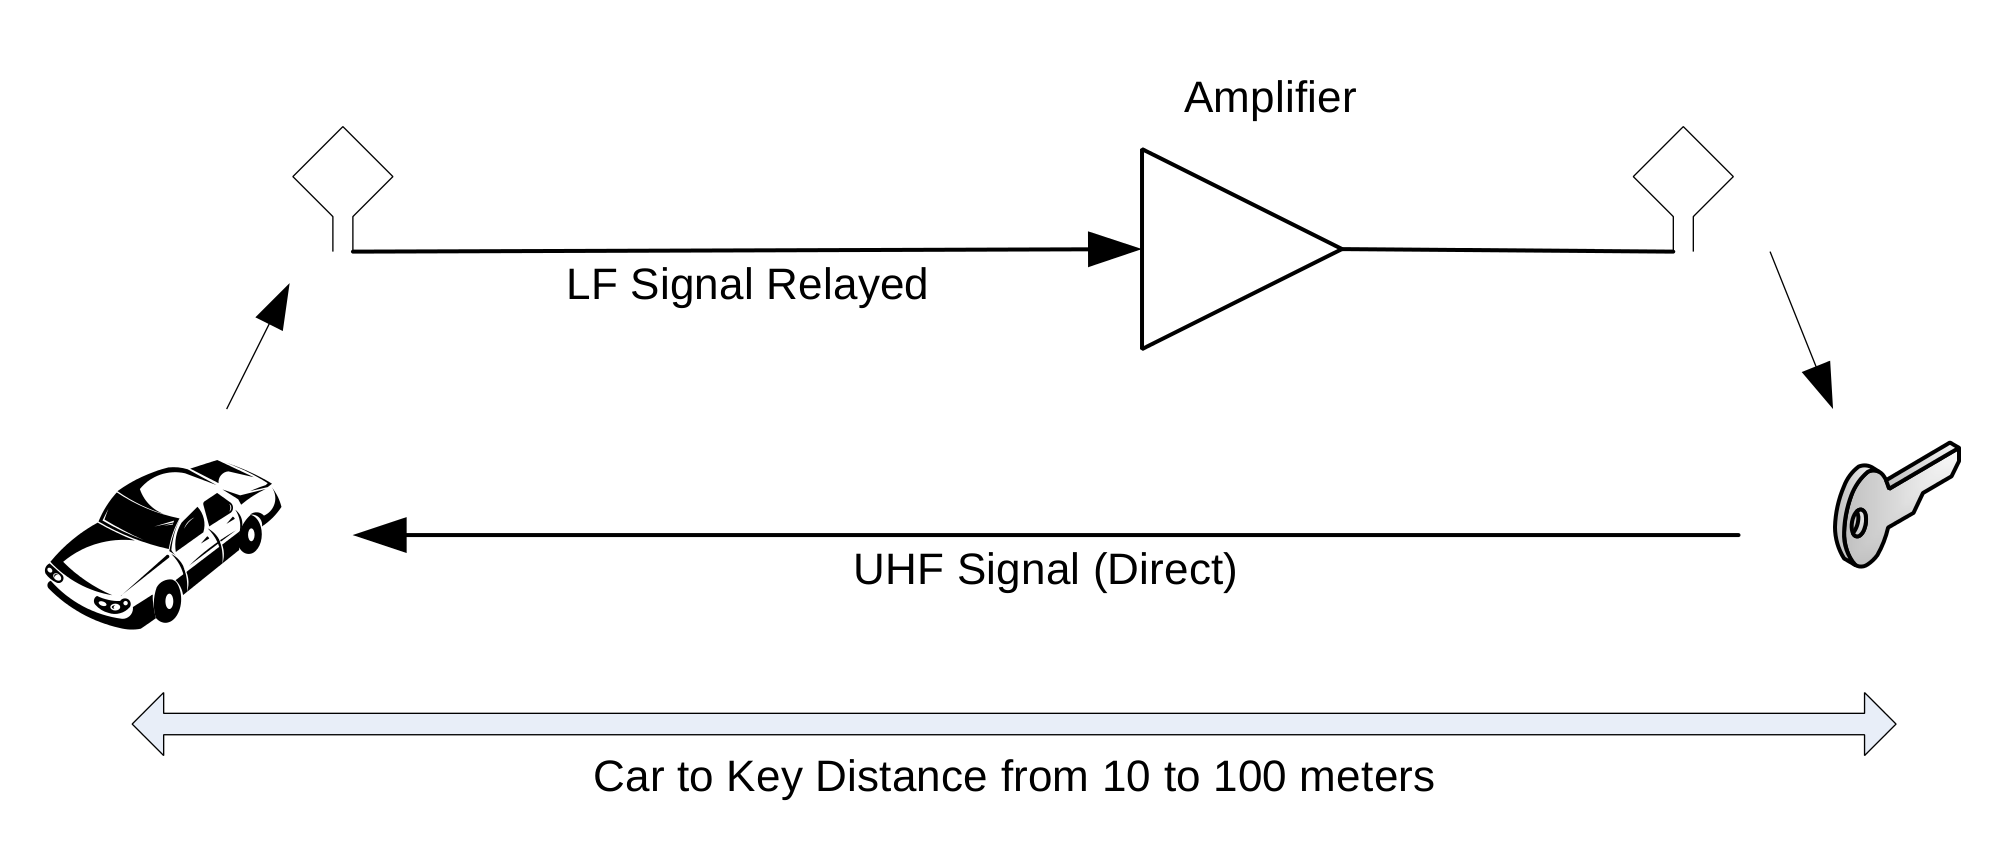
\includegraphics[width=\textwidth]{pictures/franc_relay_over_the_wire.png}
		\end{center}
		\caption{Relay wih antennas, cable and amplifiers \citep[p. 5]{relayAttacksFranc}.}
		\label{fig:relayOTW}
	\end{figure*}

	Relay  attacks on PKE systems can be carried out in different ways.
	In the most simple case,
	a cable is used to relay the transmitted LF signal from the car near the CID.
	An Amplifier might be needed to keep the signal stron enough.
	The keys UHF sender is strong enough so that the car will receive the send out signals.
	This case is shown in Figure \ref{fig:relayOTW}.
	Amplifiers might be nesscessary deping on the length of the cable,
	the quality of the antennas and the strength of the signal.

%Over the air
	\begin{figure*}[t]
		\begin{center}
			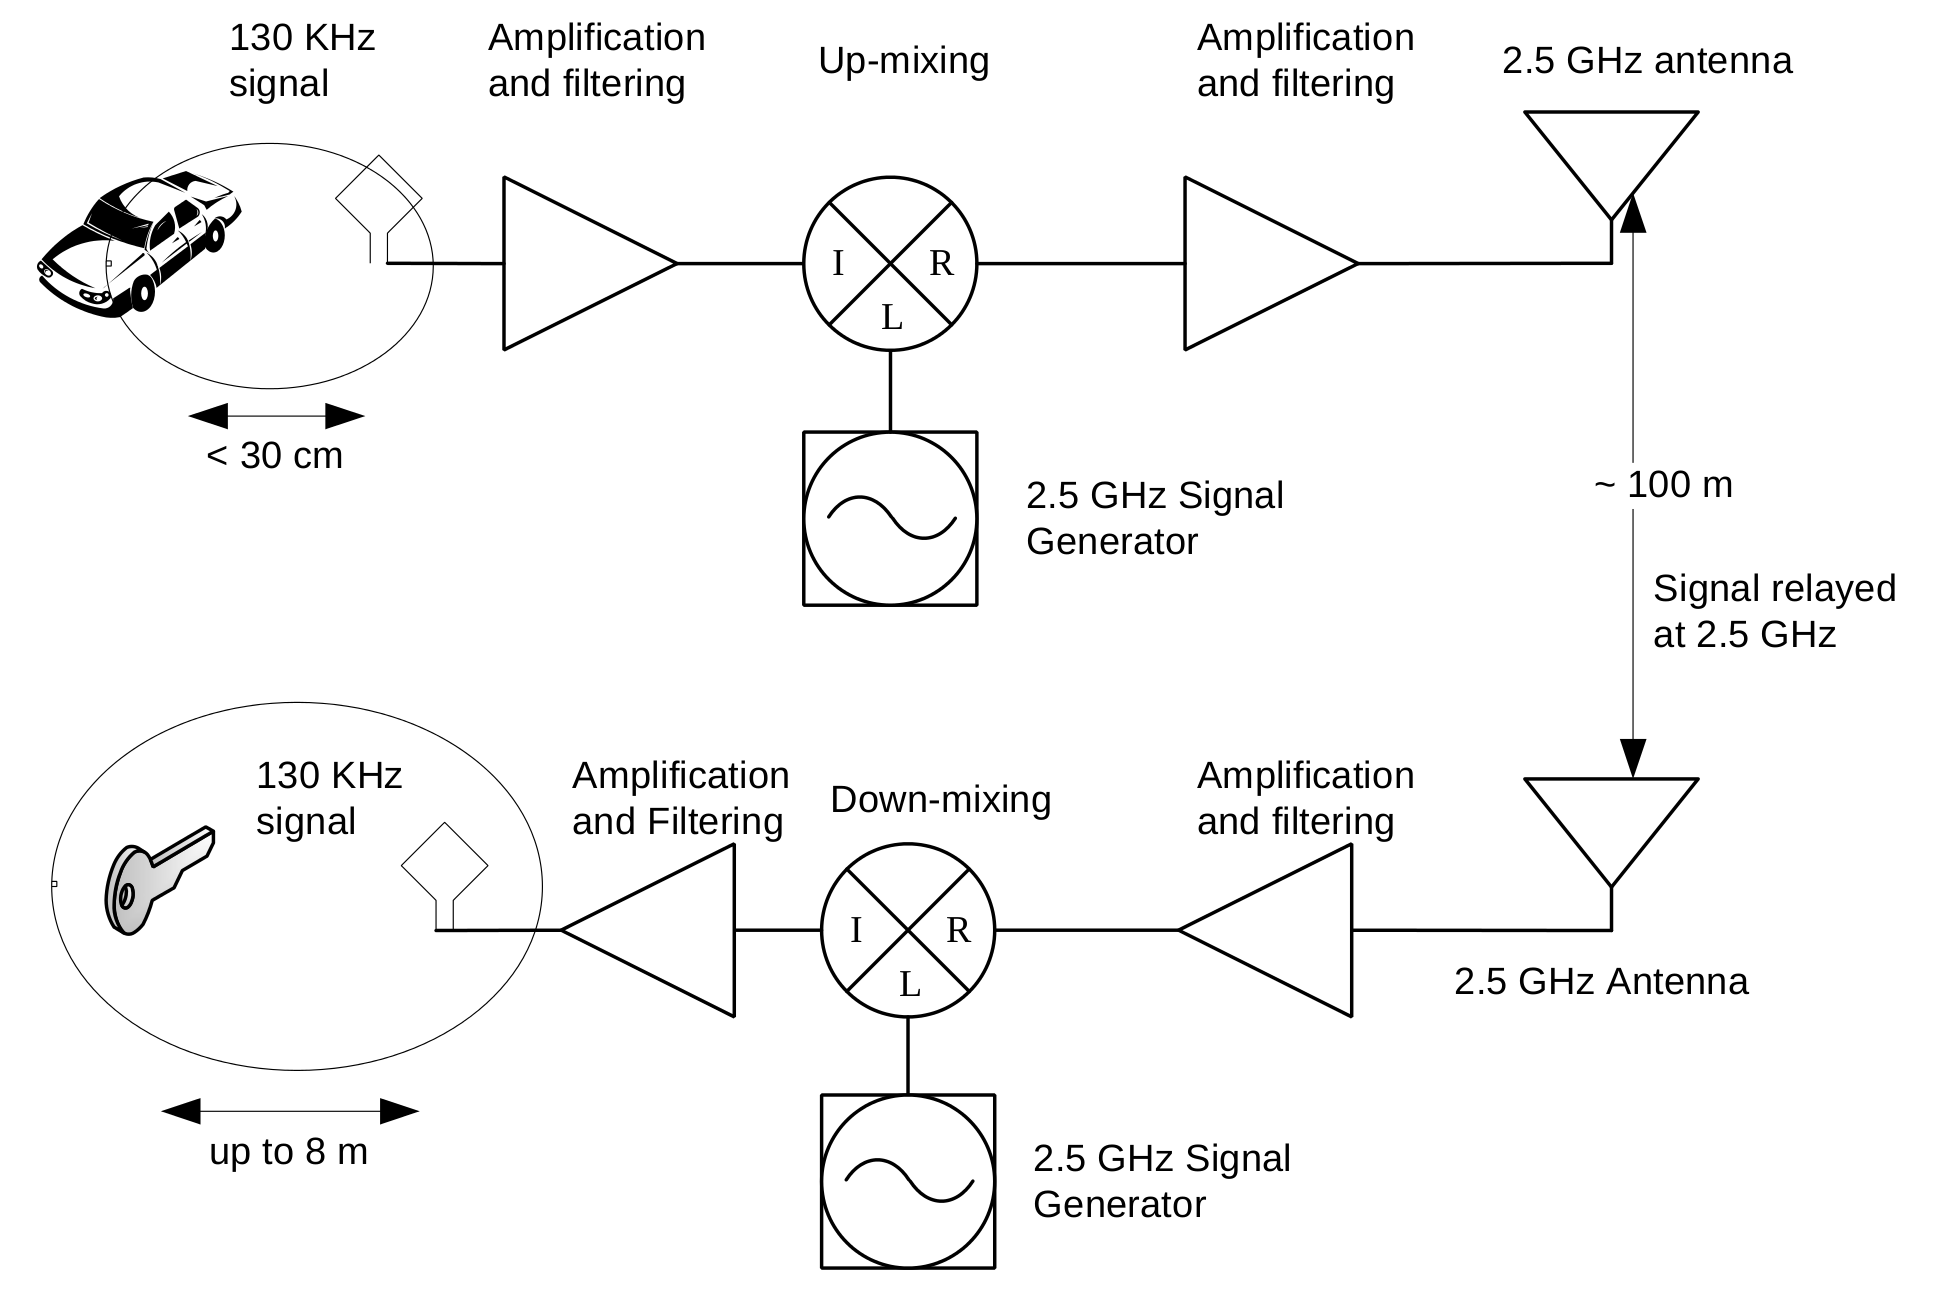
\includegraphics[width=\textwidth]{pictures/franc_relay_over_the_air.png}
		\end{center}
		\caption{Relay over-the-air with up- and downconversion and amplifiers \citep[p. 6]{relayAttacksFranc}.}
		\label{fig:relayOTA}
	\end{figure*}
	A cable is rather impractical to relay the signal.
	\citeauthor{relayAttacksFranc} used upconversion and downconversion to realy the signal.
	The 130 kHz signal transimetted by the car is amplified and upconverted to a 2.5 GHz signal.
	This signal is send out to a 2.5 GHz antenna and downmodulated to 130 KHz again.
	Amplifiers are used as required by signal strength and quality.
	The conversion steps are down analog,
	to ensure a fast conversion rate.
	Also this keeps the attack simple and inexpensive.
	Figure \ref{fig:relayOTA} show the layout of the Relay over-the-air attack.
	The Materials required for the over the air attack are rather cheap,
	an a device cloud be build for less than thousand US-Dollars.  %TODO get a reference for that

%Distance to CID
	In addition the \citeauthor{relayAttacksFranc} tested the maximum distance
	the relaying antenna can have to the CID.
	This Variable greatly determines the pracicability of the attack.
	If you have to get to close to the owner carrying his CID,
	it may raise suspicion.

%Timings
	The PKE systems use a mechanism to discriminate between signals in time.
	\citeauthor{relayAttacksFranc} tested the maximum delay that could be added
	so that the relay attack would still be succesful.
%Cars
	\citeauthor{relayAttacksFranc} acqiured 10 distinct car models that have been build by 8 different manufacturers,
	to test the raly attack in practice.
	The cars were from different classes,
	there were 4 executive or luxury class cars, 2 SUVs, a minivan and 2 cars in the compact class.
	One of the cars had an aftermarket PKE systems.
	The authors tried to attack these ten systems with both,
	the over-the-air and the over-the-cable attack.

\subsubsection*{Results}
%results francillion et al. achieved with real world cars
	The Authors were able to succesfully carry the attack out to various number of cars.
	These models were tested if they were vulnerable against the two thieves attack as described in 
	Section \ref{par:twoThieves}.
	\citeauthor{relayAttacksFranc} were able to excite the CID from ranges up to 8 meters
	and therefore open the car altough the car was more than 50 meters away.

%relay distance cable
	All of the Cars could be opened and started using the relay over-the-cable attacks in a range of 7 Meters.
	Except for one model,
	all cars could be driven away with altough the CID was 30 meters away.
	If the signals were relayed 60m,
	six out of ten cars could opened and started.
	Three of these six did not require an amplification of the signal.
	The missing cars were not tested by the authors in these distances.

%relay distance CID antenna
	\citeauthor{relayAttacks} also tested the maximum distance from the relaying antenna to the CID.
	Without amplification amplification the shortest maximum distance to allow the opening of the vehicle was 10 cm,
	the largest was 2.5 meters.
	To start the engine the lowest distance was 10 cm and the longest distance was 2.4 meters.
	With amplification of the signal the lowest distance was 2.4 m to start and to ignite the engine.
	These values were achieved on a car where the distance for opening and starting the engine were 10 cm
	without amplifying the signal.
	The Maximum distance achieved to open and start the engine achieved,
	was 8 meters
	
	\begin{table*}[t]
		\centering
		\begin{tabular}{ p{2.6cm} r l r l r l}
			\toprule
			Car model	&	\multicolumn{2}{l}{Maximum Delay}	&	\multicolumn{2}{l}{Key Response (std dev)}	&	\multicolumn{2}{l}{Key Response Time Spread}\\
			\midrule
					1 		&	500 			&\textmu s	&	1782  &	\textmu s		(\textpm 8)	&	21		&\textmu s \\
					2 		&	5000			& \textmu s	&	11376 & \textmu s  (\textpm 15)		&	47		&\textmu s \\
					4 		&	500 			&\textmu s	&	-		&										&	- 		&	\\
					5 		&	1000			& \textmu s	&	5002	& \textmu s  	(\textpm 4)		&	11		&\textmu s \\
					6 		&	10000-20000	& \textmu s	&	23582 & \textmu s 	 (\textpm 196)	&	413	&	\textmu s \\
					7 		&	620 			&\textmu s	&	1777	& \textmu s  	(\textpm 12)	&	25		&\textmu s \\
					8 		&	620 			&\textmu s	&	437	& \textmu s  	(\textpm 70)	&	162	&	\textmu s \\
					9 		&	2000			& \textmu s	&	1148	& \textmu s  	(\textpm 243)	&	436	&	\textmu s \\
					10 	&	35 			& \textmu s	&	2177	&\textmu s  	(\textpm 8		&	12		&\textmu s \\
			\bottomrule
		\end{tabular}
		\caption{Experimentally tested maximum delay, key response time and spread per model, from \cite{relayAttacksFranc}}
		\label{tab:francTimings>}
	\end{table*}

\subsection*{Implications}
% "The Supermarket"
\subsubsection*{Stealing}
	\label{sec:attackImplications}
	Relay attacks can be carried out by very simple devices,
	and can be succesfully applied.
	A typical scenario could be on a supermarket car lot.
	Two thieves steal a car locked by a PKE system.
	The owner carries his CID into the supermarket where the first thief gets close to him.
	Using the devices described in Section \ref{sec:matmet} as relay-over-the-air.
	The second thief is close by the car they want to steal.
	The thieves carry their antennas close to the car and the CID so that the vehicle will open
	and the engine ignites.
	Without notice both thieves can get away then.

	A very similar attack was tested by \citeauthor{relayAttacksFranc}.
	The Authors were able to open and start a car using the relay-over-the-cable 
	attack on a car parked in front of a buereau building.
	The CID was in bag close to the window,
	so that amplification of the signal was enough to excite the key.
	The car opened and the attackers were able to drive away.

%ODB-II
	\subsubsection*{Flaws in car security}
	Gaining access to a vehicle has further implications for the overall security of a car.
	Stealing the car is the straightforward approach,
	but in combination with attacks on the cars internal electronic system,
	malvolent attacks on the vehicle and its passenger are possible.

	Modern vehicles are controlled by many small electronic computing units (ECU),
	whom are interconnected over a bus system.
	Prominent ECUs manage the engine, the breaks or the Electronic devices on the dasboard.
	The more security relevant ECUs are connected via a priviledged,
	high-speed bus,
	where less important ones use a seperate lower-speed bus.
	These bus-systems should be strictly seperate as specified in the standard. %TODO cite standard for OMB-II
	Seperating the communication of the brakes and windscreenwipers,
	shall ensure that the integral systems keep working,
	when it is acceptable that less important ones can fail.

	However the article form \citeauthor{expModernAuto}
	shows that these security features and the standards were not implemented as intended.
	The authors also show what can be done,
	if access to the electronic bus system can be achieved.
	They tested these attacks on a closed runway with
	and were able to verify the results they gained on a jacks in a realistic setting.
	Given access to the ODB-II port of the attacked car,
	they were able to controll and shutdown ECUs.
	From less security relevant settings like honking the horn or
	engaging the windescreen whipers to life threatening attacks were possible.

	For example the engine ECU could be set in a special update mode,
	which instantly cuts the engine even while driving.
	This is an example for a major deviation from the standard,
	which clearly states that this should not be possible under any given circumstances.
	Another example is the possebility to engage the breaks on single wheels,
	or increasing the engines RPM.

	These lifethreatening attacks are possible on the car that \citeauthor{expModernAuto} tested.
	The authors also point out that,
	it is not possible to traceback certain attacks,
	as the ECUs can be reseted.

	%what harm can occur from gaining unnotices acces to the vehicle
